\begin{frame}{Percepción Remota}
    \begin{block}{¿Qué es la percepción remota?}
        Técnica o conjunto de técnicas que permite medir y registrar la energía
        electromagnética reflejada o emitida por la superficie de la Tierra y 
        relacionar tales mediciones con su naturaleza y distribución.
    \end{block}    

    Consta de tres elementos:
    \begin{itemize}
        \item Fuente de iluminación
        \item Sensor
        \item Objeto observado
    \end{itemize}
\end{frame}

\begin{frame}{Tipos de sensores}
    \begin{itemize}
        \item Sensores pasivos.- no poseen una fuente de energía por lo que solo detectan la radiación emitida y/o reflejada por la superficie terrestre que proviene de una fuente externa (como el la luz del sol).
        \item Sensores activos.- poseen una fuente propia de energía que les permite emitir su propia radiación la cuál interactúa con la superficie terrestre y al ser reflejada es captada por el sensor.
    \end{itemize}
    
    \begin{figure}
        \centering
        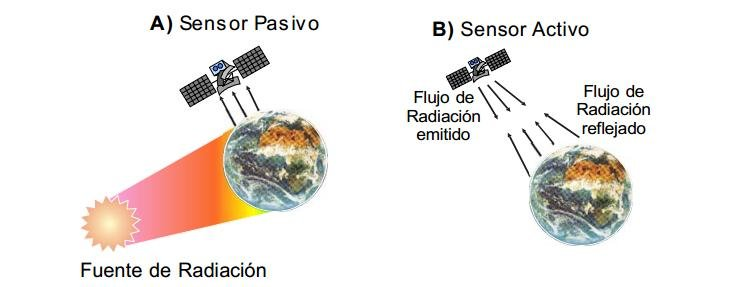
\includegraphics[scale=0.4]{img/section_03/tipos_de_sensores.png}
        \caption{Sensores activos y sensores pasivos \cite{phdthesis}}
        \label{fig:section_03_sensores_activos_pasivos}
    \end{figure}
\end{frame}

\begin{frame}{Espectro eletromagnético}
    \begin{figure}
        \centering
        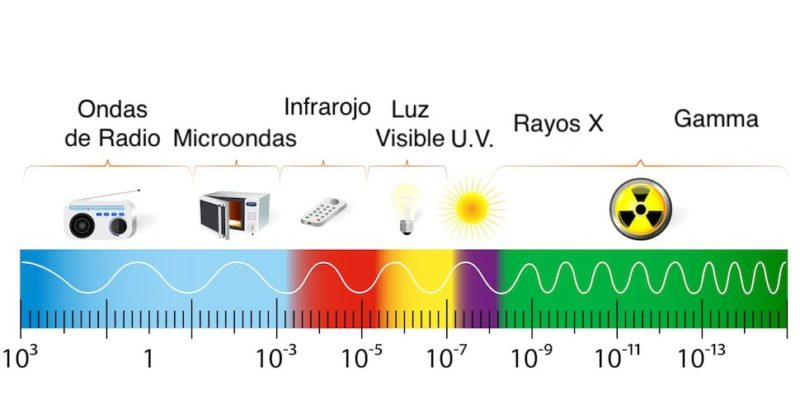
\includegraphics[scale=0.2]{img/section_03/espectro-electromagnetico.jpg}
        \caption{Espectro electromagnético}
        \label{fig:section_03_espectro_electromagnetico}
    \end{figure}
    
    \tiny
    \begin{table}
        \centering
        \begin{tabular}{c|c|c}
            \hline
            Banda & Longitud de onda & Tipo de Instrumentos \\
            \hline
            Radar & 1-30 cm & SLAR/SAR \\
            Microondas & 2-8 mm & Radiómetros \\
            Infrarojo termal & 1-14 um & Videocámaras y escáner de línea \\
            Infrarojo (MIR) & 3-5 um & Videocámaras y escáner de línea \\
            Bajo infrarojo & 1-3 um & Filme y videocámaras \\
            Visual & 350-750 nm & Filme, videocámaras y espectrómetros \\
            Ultravioleta & 250-350 nm & Filme, videocámaras y escáner de línea
            \hline
        \end{tabular}
        \caption{Bandas en detección remota}
        \label{tab:bandas_deteccion_remota}
    \end{table}
\end{frame}

\begin{frame}{Resolución}
    \footnotesize
    
    La resolución de un sensor es su habilidad para registrar información en detalle de las distintas cubiertas. La resolución depende de la capacidad de los sensores para distinguir variaciones de la energía electromagnética, del detalle espacial que captura y del número y ancho de las bandas que alberga.
    
    \begin{itemize}
        \item Resolución espacial.- es el objeto más pequeño que puede ser distinguido sobre la imagen. Define el tamaño del píxel, que es la distancia correspondiente al tamaño de la mínima unidad de información en la imagen.
    
        \item Resolución espectral.- es el número y el ancho de las bandas espectrales que puede discriminar el sensor, monoespectrales y multiespectrales.
    
        \item Resolución radiométrica.- es la capacidad para detectar variaciones en la radiancia espectral que recibe. Determina el número de niveles de gris recogidos y se expresa en niveles por píxel. A mayor resolución radiométrica, mejor interpretación de la imagen.
    
        \item Resolución temporal.- es la periodicidad con que el sensor adquiere imágenes de la misma porción de la superficie terrestre. Esta en función de las características orbitales de la plataforma (altura, velocidad e inclinación) y del diseño del sensor (ángulo de observación y ángulo de cobertura).
    \end{itemize}
\end{frame}

\begin{frame}{Radar de Apertura Sintética}
    \footnotesize
    
    \begin{itemize}
        \item Sensor activo.- emite microondas ($f_0 = 1-30 Ghz$) con cierto ángulo de incidencia ($\theta_i = 20-65°$) y forma imágenes con el eco $\sigma^0$ de la radiación emitida.

        \item Apertura sintética.- integra la historia de $\sigma^0$ durante un cierto tiempo $T_i$ a lo largo de la trayectoria de vuelo del sensor y con ello \textit{sintetiza} una antena $L_{SAR} >> L_{real}$

        \item Formación de la imagen.- basada en el principio de retrodispersión de las microondas por parte de las ondas de Bragg.
    \end{itemize}

    \begin{figure}
        \centering
        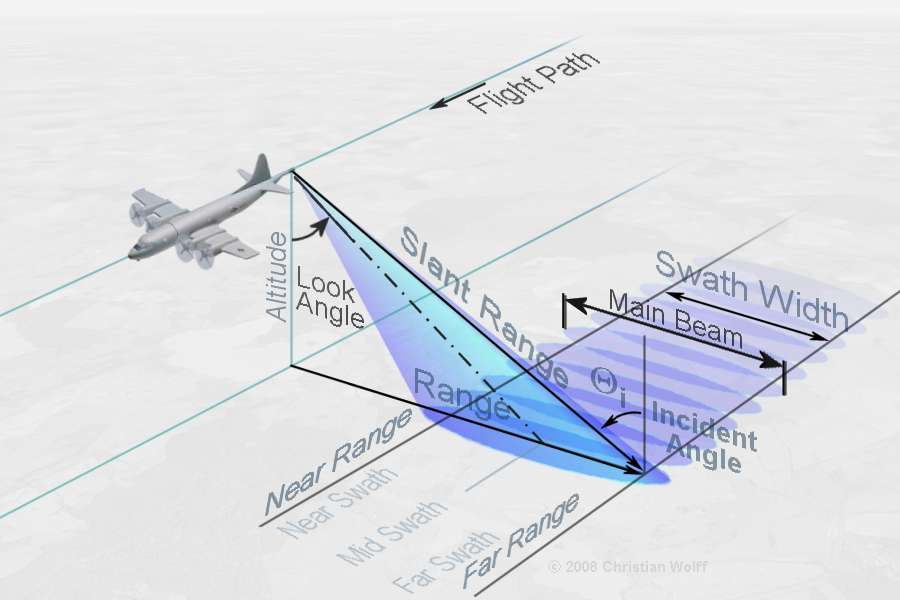
\includegraphics[scale=0.2]{img/section_03/SLAR-geometry_p.jpg}
        \caption{Radar de apertura sintética}
        \label{fig:section_03_radar_apertura_sintetica}
    \end{figure}
\end{frame}

\begin{frame}{Dinámica de la interacción SAR-Derrame}
    \begin{figure}
        \centering
        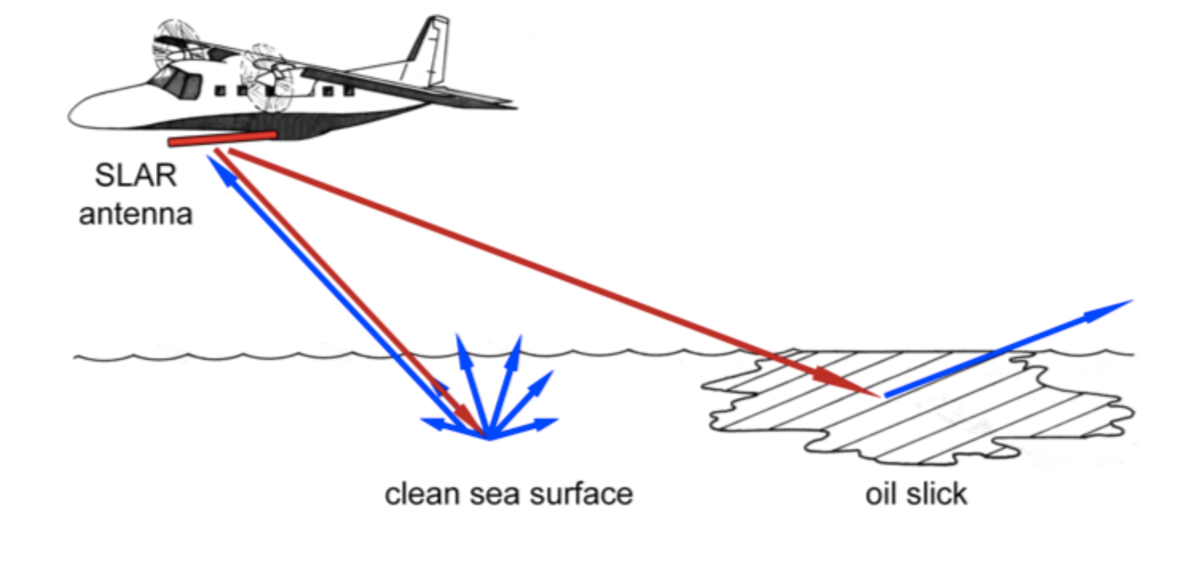
\includegraphics[scale=0.2]{img/section_03/sar-petroleo.png}
        \caption{Dinámica de la interacción entre el pulso del radar y la superficie del derrame de petróleo}
        \label{fig:section_03_dinamica_sar_petroleo}
    \end{figure}
\end{frame}
